\section{Recursive Methods \& Data Structures}

Rekursive metoder er metoder, som kalder sig selv. Rekursion kan i nogle tilfælde gøre kodestykker meget kortere og være meget lettere at implementere end iteration (fx Koch-kurver). Derimod kan rekursion nemt være meget langsommere, og nogle gange fylde meget mere i hukommelsen, hvis man ikke er varsom.

\subsection{Fibonacci}

\begin{itemize}
  \item Fibonacci-tallene er et godt eksempel på en noget som kan defineres som en rekursiv funktion. Sekvensens definition siger, at hvert nyt tal i sekvensen er summen af de to foregående tal, og de to første tal er begge 1. Kvadrater med sidelængde af disse tal kan sættes op omkring hinanden i spiraler. 
  \begin{itemize}
    \item Sekvensen ser således ud: 1, 1, 2, 3, 5, 8, 13, 21, 34, etc.
    \item $1+1=2$, $2+1=3$, $3+2=5$, $5+3=8$, etc.
  \end{itemize}

  \item Rekursivt kan metoden defineres således:
  \[
    F_n =
    \begin{cases}
      1                 & n \in \{1,0\} \\
      F_{n-1} + F_{n-2} & n > 1
    \end{cases}
  \]
  \item Man kan skrive en tilsvarende metode i Java således:
  \begin{itemize}
    \item
      \begin{verbatim}
    public int fib(int n) {
        if (n == 0 || n == 1)
            return 1;
        return fib(n-1) + fib(n-2);
    }
      \end{verbatim}
    \item Testen for om n er 0 eller 1 kaldes en stopbetingelse. En rekursiv metode bør altid have en stopbetingelse, så man er sikker på, at den ikke fortsætter med at kalde sig selv uendeligt.
  \end{itemize}

  \item Rekursive kald giver anledning til visualisering vha. træstrukturer. For et kald til fib(4) laves to yderligere kald, fib(3) og fib(2), og hver af disse kald laver yderligere to kald, etc. Følgende træstruktur viser kaldet til fib(4):

  \Tree [.fib(4)  [.fib(3)
                      [.fib(2) 
                          [.fib(1) ]
                          [.fib(0) ] ]
                      [.fib(1) ] ]
                  [.fib(2) 
                      [.fib(1) ]
                      [.fib(0) ] ] ]
  \item Bemærk, at fib(2) og fib(0) kaldes to gange, mens fib(1) kaldes tre gange. Dette er et perfekt eksempel på en langsom/ineffektiv implementation, hvor de samme værdier beregnes flere gange.
\end{itemize}

\subsection{Fraktaler}

\begin{itemize}
  \item Fraktaler er rekursiv grafik. Fraktaler er kurver som aldrig er glat nok til at kunne approximeres med linjestykker. Hvis man “zoomer ind” på en fraktal vil den altid “udfolde sig” mere. Velkendte fraktaler inkluderer Mandelbrot-mængden, Sierpinski-trekanter og Koch-linjer.
  \begin{itemize}
    \item En Koch-linje er et linjestykke med et “trekantet hak” i midten, som gør at hvert linjestykke brydes ned i fire linjestykker, som hver brydes ned i fire linjestykker, osv.
    
    \begin{center}
      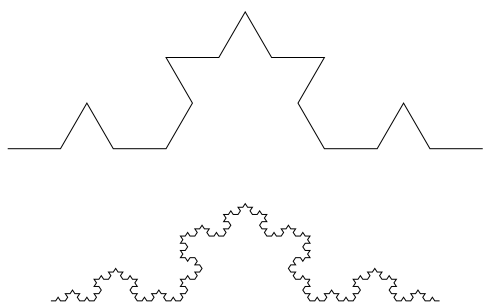
\includegraphics[scale=0.7]{images/koch_line.png}
    \end{center}
    
    \item Koch-linjen kan defineres rekursivt vha. et “tegneobjekt”, fx et Crayon objekt $c$, hvis \verb|turn(x)| metode drejer objektet $x$ grader, og \verb|move(y)| tegner en streg af længde $y$.
    \begin{verbatim}
      private void kochLine(int order, double len) {
          // Stopkriterie
          if (order == 0) c.move(len);
        
          // Rekursionsskridt
          kochLine(order-1,len/3); c.turn(-60);
          kochLine(order-1,len/3); c.turn(120);
          kochLine(order-1,len/3); c.turn(-60);
          kochLine(order-1,len/3);
      }
    \end{verbatim}
    \item Hvis stopbetingelsen ikke er opfyldt vil hvert kald til kochLine lave 4 rekursive kald. Det bliver derfor meget hurtigt kompliceret manuelt at gennemløbe sådan en metode, og træstrukturen vil blive meget bred, meget hurtigt.
  \end{itemize}
\end{itemize}

\subsection{Evaluering af udtryk}

\begin{itemize}
  \item Rekursion kan bruges til evaluering af matematiske udtryk. Man kan have et udtryk som $3+4*5$, som ikke beregnes “lineært”. Her kan man opdele de matematiske udtryk i forskellige elementer.
  \begin{itemize}
    \item Operatorer
    \item Deludtryk, som kan være enten et tal eller endnu et deludtryk
    
    \begin{center}
      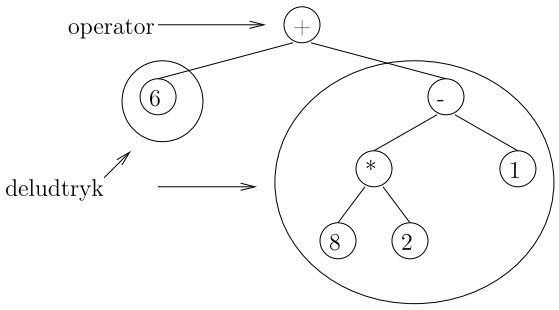
\includegraphics[scale=0.7]{images/syntax_tree_math.png}
    \end{center}
    
  \end{itemize}
  
  \item På den måde vil en metode, fx \verb|getValue(String exp)| kalde sig selv rekursivt, hver gang den har brudt et udtryk ned i to deludtryk. Når deludtrykkene til sidst udmunder i tal bliver der langsomt returneret delværdier, indtil hele udtrykket er beregnet.
  
    \begin{center}
      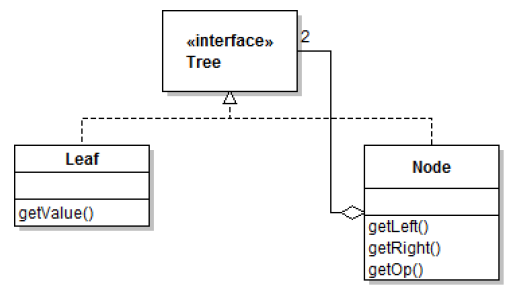
\includegraphics[scale=0.8]{images/composite_pattern.png}
    \end{center}
  
\end{itemize}

